\documentclass[border=5pt]{standalone}
\usepackage{tikz}
\usepackage{xcolor}
\usetikzlibrary{calc,shadows.blur}

% J7 - Blue flat washer
\begin{document}
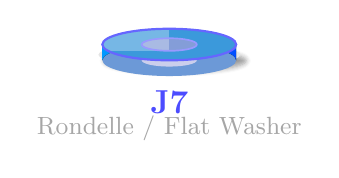
\begin{tikzpicture}

% Shadow
\fill[gray!20,blur shadow={shadow blur steps=5}] (0,-0.05) ellipse (0.9 and 0.14);

% Bottom ellipse outer
\fill[cyan!50!blue!60] (0,-0.12) ellipse (0.85 and 0.2);
\fill[cyan!30!blue!20] (0,-0.12) ellipse (0.35 and 0.08);

% Side wall (thin - washer is flat)
\fill[left color=cyan!60!blue, right color=cyan!30!blue]
  (-0.85,-0.12) -- (-0.85,0.08) arc[start angle=180,end angle=0,
  x radius=0.85, y radius=0.2] -- (0.85,-0.12)
  arc[start angle=0,end angle=180, x radius=0.85, y radius=0.2];

% Inner hole side
\fill[cyan!20!blue!30]
  (-0.35,-0.12) -- (-0.35,0.08)
  arc[start angle=180,end angle=0, x radius=0.35,y radius=0.08]
  -- (0.35,-0.12)
  arc[start angle=0,end angle=180, x radius=0.35, y radius=0.08];

% Top face outer
\fill[cyan!70!blue!80] (0,0.08) ellipse (0.85 and 0.2);
\fill[cyan!40!blue!50] (0,0.08) ellipse (0.35 and 0.08);

% Highlight
\begin{scope}
  \clip (0,0.08) ellipse (0.85 and 0.2);
  \fill[white,opacity=0.3] (-0.9,0.0) rectangle (0.0,0.32);
\end{scope}

% Outlines
\draw[blue!60, line width=0.8pt] (0,0.08) ellipse (0.85 and 0.2);
\draw[blue!40, line width=0.6pt] (0,0.08) ellipse (0.35 and 0.08);

% Label
\node[font=\bfseries\large, text=blue!70] at (0,-0.65) {J7};
\node[font=\small, text=gray!70] at (0,-0.98) {Rondelle / Flat Washer};

\end{tikzpicture}
\end{document}
